\documentclass{beamer}
\usetheme{Bergen}
\usecolortheme{seagull}
\usepackage{verbatim}

\title{dzenstat}
\author{ayekat}
\date{\today}

\begin{document}

\maketitle

\begin{frame}
  \begin{center}
    
\includegraphics[height=.8em]{img/dzenstat1.png}\\
    
\includegraphics[height=.8em]{img/dzenstat2.png}\\
    
\includegraphics[height=.8em]{img/dzenstat3.png}
  \end{center}
\end{frame}

\begin{frame}
  \frametitle{about}
  \begin{itemize}
    \pause\item System monitor for dzen2
    \pause\item RAM, CPU, network IF, battery, volume, date\,\&\,time
  \end{itemize}
\end{frame}

\begin{frame}
  \frametitle{but\,\dots}
  \pause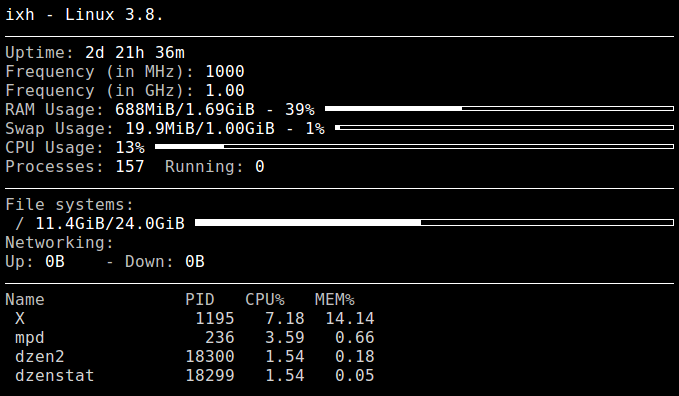
\includegraphics[width=\textwidth]{img/conky.png}
\end{frame}

\begin{frame}[fragile]
  \frametitle{why?}
  \pause
  \begin{verbatim}${execi 1 muted.sh}\end{verbatim}
  with \textbf{muted.sh:}
  \begin{verbatim}
[ $(amixer get Master | tail -n 1 | \
    awk '{print $6}') = "[off]" ] \
    && echo 1 || echo 0
  \end{verbatim}
\end{frame}

\begin{frame}[fragile]
  \frametitle{why not simply patch conky?}
  \begin{itemize}
    \pause\item NIH ;-)
    \pause\item no, seriously, no clue about coding
    \pause\item learn a lot of things
    \begin{itemize}
      \pause\item \verb+select()+, netmon, inotify,\,\dots
    \end{itemize}
  \end{itemize}
\end{frame}

\begin{frame}[fragile]
  \frametitle{todo}
  \begin{itemize}
    \pause\item polling (ALSA \verb+snd_mixer_set_callback()+)
    \pause\item too much sh in C
  \end{itemize}
\end{frame}

\end{document}

